\documentclass[12pt,a4paper]{article}
\title{MATH1110 Lec 009 Week 6-W}
\author{Benjamin Thompson}
\date{September 29, 2021}

\newcommand{\vspaceC}{\vspace{4cm}}
\usepackage[left=2cm,right=2cm]{geometry}

\usepackage{tikz, tikz-3dplot}
\usetikzlibrary{arrows.meta,decorations.markings}
\usepackage{etoolbox}

\usepackage{pgfplots}

\pgfplotsset{every axis/.append style={
axis x line=middle,    % put the x axis in the middle
axis y line=middle,    % put the y axis in the middle
axis line style={-{Stealth[length=3mm]},color=black}, % arrows on the axis
minor tick num=1
}}

\usepackage{amsmath}
\usepackage{graphicx}

\usepackage{fancyhdr}
\pagestyle{fancy}

\fancyhf{}
\lhead{MATH1110 Sec 009}
\chead{Week 6-W}
\rhead{September 29, 2021}
\cfoot{}

\begin{document}
\subsection*{Practice Quiz}
\begin{enumerate}
    \item Evaluate
    \[
        \lim_{x \rightarrow 0} \frac{(1-\cos x)(1+\cos x)}{x}
    \]
    if it exists. If it does not, explain why.
    \vspaceC
    \item Find all values $a$ for which the tangent line to the curve $y = x(x+1)^2$ at $x=a$ is horizontal.
    \vspaceC
    \item Let $f(x) = \sin(x)/x$ when $x \ne 0$, and $f(0) = 1$. Is $f$ differentiable at $x=0$?
   % \item Does $(pq)' = p'q'$ for all polynomials $p(x),q(x)$? If not, give a pair of polynomials $(a(x),b(x))$ for which $(ab)' \ne a'b'$. 
    \vspaceC
    \item Does $(pq)' = p'q'$ for any polynomials $p(x),q(x)?$ If so, give a pair of polynomials $(a(x),b(x))$ for which $(ab)' = a'b'$.
    \vspaceC
\newpage
\lhead{Name:}
    \item A polynomial $p(x)$, as well as its derivative $p'(x)$ and second derivative $p''(x)$ are plotted below. Match $p,p',p''$ with $A,B,C$.
\[
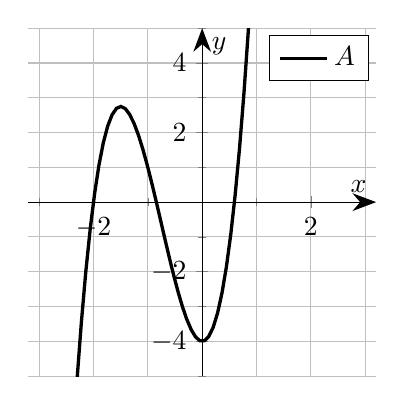
\begin{tikzpicture}
\begin{axis}[xlabel={$x$},ylabel={$y$},width=6cm, height=6cm, xmin=-3.2,xmax=3.2, ymin=-5,ymax=5, grid=both]
\addplot [very thick, domain=-4:4,samples=100]{4*x^3 + 9*x^2 - 4};
\addlegendentry{$A$}
\end{axis}
\end{tikzpicture}
\quad
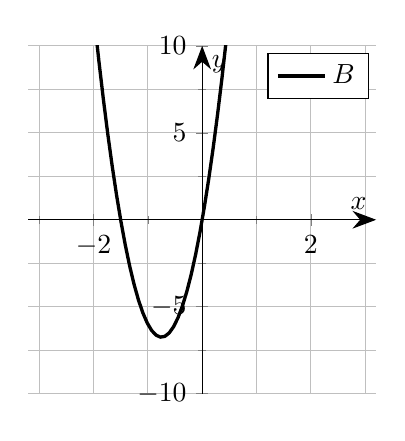
\begin{tikzpicture}
\begin{axis}[xlabel={$x$},ylabel={$y$},width=6cm, height=6cm, xmin=-3.2,xmax=3.2, ymin=-10,ymax=10, grid=both]
\addplot [very thick, domain=-4:4,samples=100]{6*x*(2*x+3)};
\addlegendentry{$B$}
\end{axis}
\end{tikzpicture}
\quad
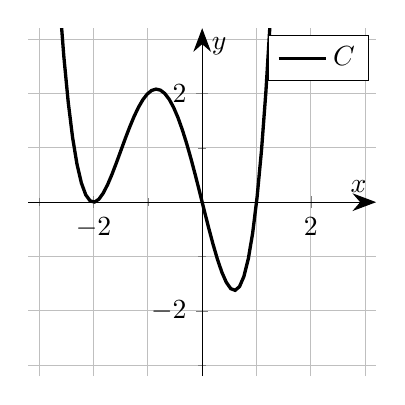
\begin{tikzpicture}
\begin{axis}[xlabel={$x$},ylabel={$y$},width=6cm, height=6cm, xmin=-3.2,xmax=3.2, ymin=-3.2,ymax=3.2, grid=both]
\addplot [very thick, domain=-4:4,samples=100]{x*(x+2)^2*(x-1)};
\addlegendentry{$C$}
\end{axis}
\end{tikzpicture}
\]
\end{enumerate}

\end{document}
